\section{Signature annotation scheme (Windows)}
\label{sign:windows}

%%%%%%%%%%%%%%%%%%%%%%%%%%%%%%%%%%%%%%%%%%%%%%%%%%%%%%%%%%%%%%%%%%%%%%%%%%%%%%%%
\subsection{Implementation}
\label{sign:windows:implementation}

\subsubsection{Interaction with the Windows Filter Engine}
\label{sign:windows:implementation:wfe}

One of the core elements that comprise our solution revolves around correctly identifying the process that generated an outgoing packet. Since this information is usually associated to the socket that performed the \texttt{send()} operation, it follows that it would be readily available at the Application Layer Enforcement (ALE) stage of the WFP Filtering Engine (see Figure \ref{sign:windows:fig:wfp}). More specifically, a callout from the \texttt{FWPM\_LAYER\_ALE\_AUTH\_CONNECT\_V4} layer is capable of blocking both outgoing TCP connections, and non-TCP traffic based on the first emitted packet.

\begin{figure}[h]
    \centering
    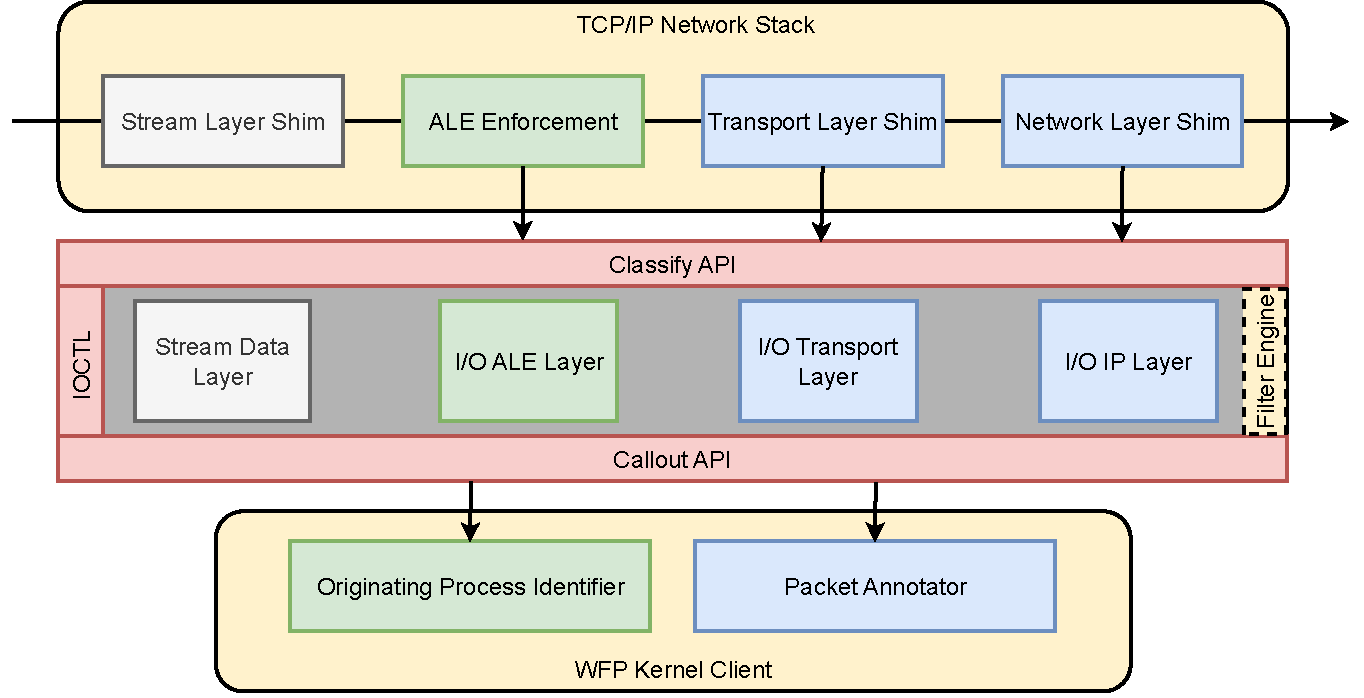
\includegraphics
        [width=1.0\textwidth, keepaspectratio]
        {figures/wfp.pdf}
    \caption{Kernel module integration with the Windows Filtering Platform.}
    \label{sign:windows:fig:wfp}
\end{figure}

Nonetheless, at this layer it is impossible to accomplish the other desired function of our firewall, namely packet annotation. The reason for this is that at the moment when the ALE hook is reached, the packet had only traversed the Stream Layer Shim of the TCP/IP network stack. If our goal was to modify the application data, doing so at the Stream / Datagram Data Layer would have been sufficient. However, our annotation scheme is reliant on the existence of network and transport layer protocol headers. Since these headers are constructed after the ALE connection management stage, we considered the \texttt{FWPM\_LAYER\_OUTBOUND\_IPPACKET\_V4} and \texttt{FWPM\_LAYER\_OUTBOUND\_TRANSPORT\_V4} layers for manipulating the IP and TCP options sections, respectively. Although these layers offer the possibility of affecting the construction of protocol headers, we note that the information relating to the originating process is no longer available at this stage.

In order to address this issue, we decided to register our Kernel Client both with the ALE layer and with the IP or Transport layers, as dictated by the user. The former callout would collect the relevant process information and attach it to the data flow as a context, thus making it available to future callouts. The latter callout would access said process information via the associated context, compute the hash-based message authentication code and attach it as an experimental option.


\subsubsection{Identification of the originating process}
\label{sign:windows:implementation:originator}

One similarity of particular note that we identified between the Windows and Linux networks stacks consists of how network traffic is attributed to a certain process. In both cases, the most accurate association can be made during the execution of the \texttt{send()} system call (or any equivalent) by assessing the PID of the calling process. However, the data that is transferred from user space during this operation can not be equated to the payload of a single packet, mainly due to mechanisms such as the Generic Segmentation Offload (i.e.: software enabled packet fragmentation). Once this data enters the network stack, its processing may be deferred to a kernel thread. Consequently, the relation of a given packet to a userspace process can be ascertained only via its backing socket structure.

Herein lies the problem. Both the \texttt{Winsock} and \texttt{sk\_buff} structures only identify one owning process: that which first instantiated the resource. However, access to said resource is granted to userspace application through file handles / descriptors, which by default are inherited by children on \texttt{exec()}. We note that aside from this, there are also other methods of sharing file descriptors between processes (e.g.: ancillary sockets that transfer file descriptors, etc.)

Our solution takes advantage of the fact that part of the processing done by the TCP/IP stack is performed by the same thread that originally invoked the \texttt{send()} operation. As a result, we are able to extract the real PID of the originating process anywhere in Stream Layer Shim or the ALE, as well as their associated Filter Engine hooks and callouts.


\subsubsection{Packet annotation}
\label{sign:windows:implementation:annotation}

Following the identification of the originating process, our system was intended to generate proof of authenticity and integrity of the payload. To this end, we utilized the BCrypt family of cryptographic primitives to calculate a SHA256 HMAC for each packet. We selected this variant instead of NCrypt due to the fact that the HMAC shared secret could be considered to have already been loaded in memory as a parameter to the kernel module. Nonetheless, we regard NCrypt as a viable alternative if the requirement of integrating a Key Storage Provider ever arises. Regardless, the digest of the Message Authentication code was calculated based on the TCP payload as well as the Sequence Number, so as to prevent replay attacks.

\begin{figure}[h]
    \centering
    \includegraphics
        [width=1.0\textwidth, keepaspectratio]
        {figures/tcp\_fw\_option.pdf}
    \caption{Experimental TCP option format used in annotation.}
    \label{sign:windows:fig:tcp-fw-option}
\end{figure}

To conclude the annotation process, we would attach the 32-byte digest to the TCP header, as a TCP option (see structure in Figure \ref{sign:windows:fig:tcp-fw-option}). Each TCP option is a Type-Length-Value (TLV) tuple that is appended to the base header and any other pre-existing options. Due to it being an experimental option (i.e., not previously registered with the Internet Assigned Numbers Association), we assigned ours the RFC3692-style \cite{rfc3692} codepoint \texttt{0xFD}. At the same time, we set the length field to the maximum value of 40 bytes. This decision was motivated by the severe space requirements of the digest, combined with additional protocol-enforced fields, and relative to the potentially variable length of other common options such as Window Scaling or Selective Acknowledgement. Because we could not guarantee that our option would be able to coexist with all the other (e.g., the aforementioned) we deemed it necessary to erase all other options present in the initial handshake for both incoming and outgoing connections. This would prevent the successful negotiation of employing any protocol extensions (aside from ours) by the operating system from that point onwards. In compliance with the Shared Use of Experiemntal TCP Options RFC \cite{rfc6994}, we assigned our experiment the ID \texttt{0x4677}. Aside from the 32-byte HMAC digest value, the Value element also consists of a 4-byte field reserved for future use. We opted for this approach instead of padding the options section with NOPs because middleboxes may remove them if encountered in groups of more than three. This truncation of the options section usually occurs since NOPs are usually employed to offset options that must be 32-bit aligned, and having a 32-bit padding sequence is not only redundant but can also be considered a type of Denial Of Service attack meant to waste system resources with TCP option decoding. Ensuring that the TCP header length is consistently 60 bytes guarantees that no other TCP options are injected on the path and simplifies the payload offset calculation process.

%%%%%%%%%%%%%%%%%%%%%%%%%%%%%%%%%%%%%%%%%%%%%%%%%%%%%%%%%%%%%%%%%%%%%%%%%%%%%%%%
\subsection{Evaluation}
\label{sign:windows:evaluation}

\subsubsection{Experimental setup}
\label{sign:windows:evaluation:setup}

Our solution was developed on a bare-metal Windows 11 Pro 22H2 and cross compiled with MSVC v143, to be tested on a Virtual Machine running Windows 10 Enterprise LTSC Build 17763, with a 1Gbps emulated network controller. The decoupling of development and testing environments was necessary for allowing the insertion of self-signed kernel modules and to minimize the risk of development setbacks.

A second Virtual Machine running Ubuntu Bionic was used to test the compliance of our annotation scheme with Linux-based distributions.

\subsubsection{Label verification and filtration}
\label{sign:windows:evaluation:linux}

In order to demonstrate the efficacy of our annotation scheme, we implemented an Xtables module for the Netfilter system in Linux. This system comprises a set of hooks placed within the network stack of the Linux kernel, and can be used to attach traffic filters and mutators. In other words, the Netfilter system represents the basis on which \texttt{iptables} was built. Correspondingly, Xtables is an aggregate name for the callback subsystem that unifies the IPv4, IPv6, ARP and Ethernet Bridge toolset backends, collectively now known as \texttt{nftables}.

Our extension also consists of a user space component (i.e., an \texttt{iptables} plugin library) that expands the parsing capabilities of the base binary to include custom match criteria and auxiliary information, such as the pre-shared secret used in the HMAC operation. This plugin marshalls the aforementioned parameters and sends them to our Xtables module, thus creating a new evaluation context, specific to a singular rule. When the \texttt{match()} callback is invoked within a certain context, our module re-calculates the SHA256-HMAC of the TCP payload and Sequence Number, compares it to that which is stored in the experimental TCP option, and finally reports the result to the caller. Since our Xtables module only implements the \texttt{match()} callback, it can be paired with any other match criteria and jump targets available to \texttt{iptables}, be they related to filtering, logging, address translation, etc.

For the purpose of testing our Linux-based filtration mechanism, we have implemented two HTTP and SSH Python servers based on \texttt{flask} and \texttt{paramiko} respectively. While the former exposed multiple routes, each providing an arbitrary implementation for different HTTP request types (e.g.: GET, POST, DELETE, etc.) the latter acted as an echo serer over a secure communication channel. We concluded that neither type of traffic was impeded by the addition of the HMAC annotation.  Additionally, we also assessed the viability of Windows-side filtration of these protocols, as well as ICMP Echo Requests / Replies and raw data over UDP but without annotating outgoing traffic.

\subsubsection{Performance considerations}
\label{sign:windows:evaluation:performance}

Despite the security assurances that our system provides, a decline in throughput is to be expected. This can be observed in Figure \ref{sign:windows:fig:throughput}, by comparing the average data throughput of ten second \texttt{iperf3} TCP transmissions, with and without annotations. These measurements have further been averaged across five different rounds of testing. Although the process identification feature is not particularly costly from a computational standpoint, calculating the SHA256 digest and replacing the contents of the send buffer by injecting the experimental TCP option can be detrimental. Based on our experiments we estimate that our kernel module imposes an upper bound of approx. 400Mbps on outgoing network transmissions. Note however that this limit may vary depending on the characteristics of the underlying testing environment (e.g., hardware implementation of cryptographic primitives, CPU frequency, etc. )

\begin{figure}[H]
    \centering
    \begin{tikzpicture}
        \begin{axis}[
            width             = \textwidth,
            height            = 8cm,
            at                = {(0,0)},
            xmin              = 0,
            xmax              = 1550,
            % ymax              = 6300,
            xtick distance    = 100,
            xticklabel style  = {rotate=45},
            xlabel            = {MTU [bytes]},
            x label style     = {at={(axis description cs:0.5,-0.175)},anchor=north},
            ylabel            = {Throughput [Mbps]},
            grid              = both,
            legend style      = {at={(0.98,0.14)}, anchor=east},
            legend cell align = left,
        ]
            \addplot[color=RoyalBlue, very thick]
                table[x=mtu, y=baseline, col sep=comma]
                {src/chapters/05-SignatureFirewall/data/throughput.csv};
            \addlegendentry{baseline}

            \addplot[color=LimeGreen, very thick]
                table[x=mtu, y=firewall, col sep=comma]
                {src/chapters/05-SignatureFirewall/data/throughput.csv};
            \addlegendentry{annotated}
        \end{axis}
    \end{tikzpicture}

    \caption{iperf3 data throughput with packet annotation.}
    \label{sign:windows:fig:throughput}
\end{figure}


